% Introduction chapter.
%
% Developed for my Master Thesis at Maastricht University.
% Based on Eugenio Senes's template at the University of Torino.
%
% By Joeri Hermans (joeri@joerihermans.com)
%
% Released under an MIT license. Share, modify and enjoy, but quote the author!

\chapter{Introduction}
\label{chapter:introduction}

In this chapter we introduce the main concept, and problems surrounding the parallization of gradient descent. We familliarize the reader with the topic and some notation by providing some context why someone would like to apply said technique. Furthermore, in Section~\ref{sec:problem_statement}, we summarize the problem statement and provide several research questions which will guide the research in this work. Finally, we conclude this chapter in Section~\ref{sec:thesis_outline} with a brief outline of the thesis.

\section{Motivation}
\label{sec:motivation}

In recent years it has been shown that being able to train large and deep neural networks result in state-of-the-art performance~\cite{wu2016google, dean2012large}, especially regarding unsupervised feature learning and image recognition. However, consider the required time, and cost of the infrastructure that would be required in order to train such a large model in a reasonable amount of time. Furthermore, it is not only the training time and cost of the infrastructure which need to be taken into consideration, but also the volume of the data. The amount of information that will be gathered will be an increasing important factor in the next few years. Not only with respect to big technology companies and government organizations, but also scientific surveys with limited budgets. These scientific surveys will generate more experimental data than ever~\cite{hllhcdesignreport, ivezic2008lsst}, and will have to process and analyze that data. To solve the problem of increased computational workloads and budget freezes, the High Energy Physics (HEP) community is exploring and researching machine learning approaches to fit physics problems~\cite{bian2016recent, de2017learning, louppe2016learning} with the intention to improve detection quality, or reduce computational constraints.\\

However, the sheer size of these datasets severly impacts the training time of the models. In order to resolve this issue, one could sample some representative subset of the data to reduce the training time. The disadvantage of this approach is that some ``diverse`` instances, i.e., data points, might not appear in the final training set. This is especially a problem in Deep Learning, where models usually benifit from having access to a lot of training data due to the high dimensionality of the parametrization~\cite{dean2012large}. To resolve this issue, Dean et al.~\cite{dean2012large} introduce two new paradigms to decrease the training time in the presence of a large dataset and a high dimensionality of the parametrization. The two paradigms, \emph{Model Parallelism}, briefly discussed in Section~\ref{sec:intro_model_parallelism}, and \emph{Data Parallelism}, discussed in Section~\ref{sec:intro_data_parallelism}, are inherently different ways of decreasing the training time of a model.\\

The first paradigm, \emph{Model Parallelism}, is intuitively the most straightforward paradigm since it deals with the parallelization of the computations within a \emph{single} model, i.e., how to parallelize the computations of a single model over multiple machines, or multiple processes. The second paradigm, which will be the main focus of this thesis, is \emph{Data Parallelism}. As stated above, the main concept of Data Parallelism will be discussed in detail in Section~\ref{sec:intro_data_parallelism}. However, for completion, think of Data Parallelism as a technique to \emph{parallelize gradient descent}. This is done by allocating $n$ processes over possibly $n$ different machines, and splitting the training set into $n$ \emph{partitions}, or \emph{data shards}. For further convenience, we will call such a process a \emph{worker}. In the next step, we assign a single distinct partition to a worker. Meaning, the worker will not be able to fetch training data from other partitions since those have been assigned to different workers. The goal of these workers is to work together, and optimize the parameters of a central model.\\

A lot of different distributed optimization schemes have been suggested in recent years~\cite{zhang2015deep, dean2012large, hadjis2016omnivore, ??}. Most of the recent contributions try to push the limits of asynchronous Data Parallelism, discussed in Section~\ref{sec:asynchronous_data_parallelism}, by simply \emph{annealing} the gradients with respect to some hyperparameter without giving a sound theoretical argument why the annealing should happen in the first place. This suggests that there is an intrinsic limit to asynchronous Data Parallelism, as suggested by~\cite{implicitmomentum}. Why not simply reduce the number of parallel workers if we reduce the impact of the gradient updates by means of annealing anyway? The approach of reducing the number of parallel workers in such a situation has been suggested by~\cite{hadjis2016omnivore}, where they perform a \emph{grid-search} of the training hyperparamers (this includes the number of workers) in order to provide the optimal hyperparameters within a training epoch. However, the disadvantage of this technique is that after every epoch, or a specific number of iterations, a grid-search of the hyperparameters has to be performed in order to obtain the optimal configuration of the hyperparameters to ensure convergence.\\

This brings us to the main motivation behind this work. We intent to obtain a better theoretical understanding of \emph{asynchronous} Data Parallism by building upon previous work, and combine it with novel insights to construct a new distributed optimization scheme without introducing new hyperparameters, or relying on grid-searches to optimize the configuration of existing hyperparameters.

\section{Model Parallelism}
\label{sec:intro_model_parallelism}

TODO

\section{Data Parallelism}
\label{sec:intro_data_parallelism}

As stated above, Data Parallelism is a technique to \emph{parallelize gradient descent}, and thereby reducing the overal training time of a model. In essence, Data Parallelism achieves this by distributing the workload over multiple workers\footnote{As stated in Section~\ref{sec:motivation}, a worker is a process on a single machine. However, it is possible that multiple workers share the same machine. Nevertheless, one could construct the distribution mechanism (even manually) in such a way every worker will be placed on a different machine.}, and by coordination the workers in such a way that they optimize the parametrization of a central model, which we denote by $\tilde{\theta}_t$. The coordination mechanism of the workers can be implemented in many different ways. However, in order to formalize the main concept of Data Parallelism, let us assume we have a dataset $D$, which contains our training data, and that we are able to distribute dataset $D$ over $n$ different workers $W = \{w_1, \ldots, w_n\}$. Where every workers holds a copy of the central model, thus, a copy of the parameterization of the central model $\tilde{\theta}_0$. Furthermore, we denote the parametrization of a particular worker $k$ at time $t$ by $\theta_t^k$. Of course, if a worker wants to contribute to the optimization of the central model, the worker needs to be able to relay update information and retrieve the most recent parameterization of the central model. This is done by instantiating a \emph{Parameter Server} (PS), where workers will be able to \emph{commit} their updates, and \emph{pull} the most recent parameterization of the central model. The parameterization of the central model is called the \emph{central variable}, which we denote by $\tilde{\theta}_t$. In the final preperation step, before the actual training starts, $D$ will be split into $n$ roughly equally sized partitions $P = \{p_1, \ldots, p_n\}$, where $\left\vert{p_i}\right\vert \approx \frac{1}{\left\vert{D}\right\vert}$. Finally, the data partition $p_i$ will be assigned to the corresponding worker $w_i$.

\begin{figure}[H]
  \centering
  % Define database shape.
  \def\database at (#1,#2){
    \draw (#1,#2) ellipse (0.5 and 0.15);
    \draw (#1 - 0.5, #2) -- (#1 - 0.5, #2 - 1);
    \draw (#1 + 0.5, #2) -- (#1 + 0.5, #2 - 1);
    \draw (#1 - 0.5, #2 - 1/3) arc (180:360:0.5 and 0.15);
    \draw (#1 - 0.5, #2 - 2/3) arc (180:360:0.5 and 0.15);
    \draw (#1 - 0.5, #2 - 1) arc (180:360:0.5 and 0.15);
  }
  % Define datashard shape.
  \def\datashard at (#1,#2){
    \draw (#1,#2) ellipse (0.5 and 0.15);
    \draw (#1 - 0.5, #2) -- (#1 - 0.5, #2 - 1/3);
    \draw (#1 + 0.5, #2) -- (#1 + 0.5, #2 - 1/3);
    \draw (#1 - 0.5, #2 - 1/3) arc (180:360:0.5 and 0.15);
  }
  % Define the neural network shape.
  \def\neuralnet at (#1,#2){
    % Draw node bounding box.
    \draw[rounded corners=3pt] (#1 - 0.7,#2 + 0.5) rectangle ++(1.4,-0.95);
    % Draw fully connected lines.
    \draw[gray] (#1 + 0.25,#2) -- (#1 - 0.375, #2 + 0.25);
    \draw[gray] (#1 + 0.25,#2) -- (#1 - 0.125, #2 + 0.25);
    \draw[gray] (#1 + 0.25,#2) -- (#1 + 0.125, #2 + 0.25);
    \draw[gray] (#1 + 0.25,#2) -- (#1 + 0.375, #2 + 0.25);
    \draw[gray] (#1 + 0.5,#2) -- (#1 - 0.375, #2 + 0.25);
    \draw[gray] (#1 + 0.5,#2) -- (#1 - 0.125, #2 + 0.25);
    \draw[gray] (#1 + 0.5,#2) -- (#1 + 0.125, #2 + 0.25);
    \draw[gray] (#1 + 0.5,#2) -- (#1 + 0.375, #2 + 0.25);
    \draw[gray] (#1,#2) -- (#1 - 0.375, #2 + 0.25);
    \draw[gray] (#1,#2) -- (#1 - 0.125, #2 + 0.25);
    \draw[gray] (#1,#2) -- (#1 + 0.125, #2 + 0.25);
    \draw[gray] (#1,#2) -- (#1 + 0.375, #2 + 0.25);
    \draw[gray] (#1 - 0.25,#2) -- (#1 - 0.375, #2 + 0.25);
    \draw[gray] (#1 - 0.25,#2) -- (#1 - 0.125, #2 + 0.25);
    \draw[gray] (#1 - 0.25,#2) -- (#1 + 0.125, #2 + 0.25);
    \draw[gray] (#1 - 0.25,#2) -- (#1 + 0.375, #2 + 0.25);
    \draw[gray] (#1 - 0.5,#2) -- (#1 - 0.375, #2 + 0.25);
    \draw[gray] (#1 - 0.5,#2) -- (#1 - 0.125, #2 + 0.25);
    \draw[gray] (#1 - 0.5,#2) -- (#1 + 0.125, #2 + 0.25);
    \draw[gray] (#1 - 0.5,#2) -- (#1 + 0.375, #2 + 0.25);
    \draw[gray] (#1 + 0.25,#2) -- (#1 + 0.125, #2 - 0.25);
    \draw[gray] (#1 + 0.25,#2) -- (#1 - 0.125, #2 - 0.25);
    \draw[gray] (#1 + 0.5,#2) -- (#1 + 0.125, #2 - 0.25);
    \draw[gray] (#1 + 0.5,#2) -- (#1 - 0.125, #2 - 0.25);
    \draw[gray] (#1,#2) -- (#1 + 0.125, #2 - 0.25);
    \draw[gray] (#1,#2) -- (#1 - 0.125, #2 - 0.25);
    \draw[gray] (#1 - 0.25,#2) -- (#1 + 0.125, #2 - 0.25);
    \draw[gray] (#1 - 0.25,#2) -- (#1 - 0.125, #2 - 0.25);
    \draw[gray] (#1 - 0.5,#2) -- (#1 + 0.125, #2 - 0.25);
    \draw[gray] (#1 - 0.5,#2) -- (#1 - 0.125, #2 - 0.25);
    % Define input layer.
    \draw[fill=white] (#1 - 0.375,#2 + 0.25) circle (1pt);
    \draw[fill=white] (#1 - 0.125,#2 + 0.25) circle (1pt);
    \draw[fill=white] (#1 + 0.125,#2 + 0.25) circle (1pt);
    \draw[fill=white] (#1 + 0.375,#2 + 0.25) circle (1pt);
    % Define hidden layer.
    \draw[fill=white] (#1 - 0.5,#2) circle (1pt);
    \draw[fill=white] (#1 - 0.25,#2) circle (1pt);
    \draw[fill=white] (#1,#2) circle (1pt);
    \draw[fill=white] (#1 + 0.25,#2) circle (1pt);
    \draw[fill=white] (#1 + 0.5,#2) circle (1pt);
    % Define output layer.
    \draw[fill=white] (#1 - 0.125,#2 - 0.25) circle (1pt);
    \draw[fill=white] (#1 + 0.125,#2 - 0.25) circle (1pt);
  }
  \def\neuralnetclean at (#1,#2){
    \draw[gray] (#1 + 0.25,#2) -- (#1 - 0.375, #2 + 0.25);
    \draw[gray] (#1 + 0.25,#2) -- (#1 - 0.125, #2 + 0.25);
    \draw[gray] (#1 + 0.25,#2) -- (#1 + 0.125, #2 + 0.25);
    \draw[gray] (#1 + 0.25,#2) -- (#1 + 0.375, #2 + 0.25);
    \draw[gray] (#1 + 0.5,#2) -- (#1 - 0.375, #2 + 0.25);
    \draw[gray] (#1 + 0.5,#2) -- (#1 - 0.125, #2 + 0.25);
    \draw[gray] (#1 + 0.5,#2) -- (#1 + 0.125, #2 + 0.25);
    \draw[gray] (#1 + 0.5,#2) -- (#1 + 0.375, #2 + 0.25);
    \draw[gray] (#1,#2) -- (#1 - 0.375, #2 + 0.25);
    \draw[gray] (#1,#2) -- (#1 - 0.125, #2 + 0.25);
    \draw[gray] (#1,#2) -- (#1 + 0.125, #2 + 0.25);
    \draw[gray] (#1,#2) -- (#1 + 0.375, #2 + 0.25);
    \draw[gray] (#1 - 0.25,#2) -- (#1 - 0.375, #2 + 0.25);
    \draw[gray] (#1 - 0.25,#2) -- (#1 - 0.125, #2 + 0.25);
    \draw[gray] (#1 - 0.25,#2) -- (#1 + 0.125, #2 + 0.25);
    \draw[gray] (#1 - 0.25,#2) -- (#1 + 0.375, #2 + 0.25);
    \draw[gray] (#1 - 0.5,#2) -- (#1 - 0.375, #2 + 0.25);
    \draw[gray] (#1 - 0.5,#2) -- (#1 - 0.125, #2 + 0.25);
    \draw[gray] (#1 - 0.5,#2) -- (#1 + 0.125, #2 + 0.25);
    \draw[gray] (#1 - 0.5,#2) -- (#1 + 0.375, #2 + 0.25);
    \draw[gray] (#1 + 0.25,#2) -- (#1 + 0.125, #2 - 0.25);
    \draw[gray] (#1 + 0.25,#2) -- (#1 - 0.125, #2 - 0.25);
    \draw[gray] (#1 + 0.5,#2) -- (#1 + 0.125, #2 - 0.25);
    \draw[gray] (#1 + 0.5,#2) -- (#1 - 0.125, #2 - 0.25);
    \draw[gray] (#1,#2) -- (#1 + 0.125, #2 - 0.25);
    \draw[gray] (#1,#2) -- (#1 - 0.125, #2 - 0.25);
    \draw[gray] (#1 - 0.25,#2) -- (#1 + 0.125, #2 - 0.25);
    \draw[gray] (#1 - 0.25,#2) -- (#1 - 0.125, #2 - 0.25);
    \draw[gray] (#1 - 0.5,#2) -- (#1 + 0.125, #2 - 0.25);
    \draw[gray] (#1 - 0.5,#2) -- (#1 - 0.125, #2 - 0.25);
    % Define input layer.
    \draw[fill=white] (#1 - 0.375,#2 + 0.25) circle (1pt);
    \draw[fill=white] (#1 - 0.125,#2 + 0.25) circle (1pt);
    \draw[fill=white] (#1 + 0.125,#2 + 0.25) circle (1pt);
    \draw[fill=white] (#1 + 0.375,#2 + 0.25) circle (1pt);
    % Define hidden layer.
    \draw[fill=white] (#1 - 0.5,#2) circle (1pt);
    \draw[fill=white] (#1 - 0.25,#2) circle (1pt);
    \draw[fill=white] (#1,#2) circle (1pt);
    \draw[fill=white] (#1 + 0.25,#2) circle (1pt);
    \draw[fill=white] (#1 + 0.5,#2) circle (1pt);
    % Define output layer.
    \draw[fill=white] (#1 - 0.125,#2 - 0.25) circle (1pt);
    \draw[fill=white] (#1 + 0.125,#2 - 0.25) circle (1pt);
  }
  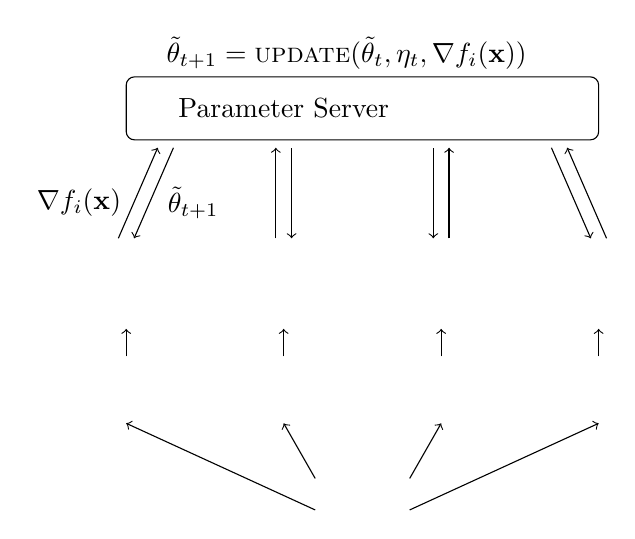
\begin{tikzpicture}
    \database at (0,0);
    \draw[->] (-0.6,-0.5) -- (-3, 0.6);
    \draw[->] (-0.6,-0.1) -- (-1, 0.6);
    \draw[->] (0.6,-0.1) -- (1, 0.6);
    \draw[->] (0.6,-0.5) -- (3, 0.6);
    \datashard at (-3,1.2)
    \datashard at (-1,1.2);
    \datashard at (1,1.2);
    \datashard at (3,1.2);
    \draw[->] (-3, 1.45) -- (-3, 1.8);
    \draw[->] (-1, 1.45) -- (-1, 1.8);
    \draw[->] (1, 1.45) -- (1, 1.8);
    \draw[->] (3, 1.45) -- (3, 1.8);
    \neuralnet at (3,2.35);
    \neuralnet at (1,2.35);
    \neuralnet at (-1,2.35);
    \neuralnet at (-3,2.35);
    % Draw the parameter server.
    \draw[rounded corners=3pt] (-3, 5) rectangle ++(6,-0.8);
    \node (pslabel) at (-1, 4.6) {Parameter Server};
    \node (psequation) at (-0.2, 5.3) {$\tilde{\theta}_{t+1} = \textsc{update}(\tilde{\theta}_t, \eta_t, \nabla f_i(\textbf{x}))$};
    % Draw the lines.
    \neuralnetclean at (1.8, 4.6);
    \draw[->] (-3.1, 2.95) -- (-2.6, 4.1);
    \draw[<-] (-2.9, 2.95) -- (-2.4, 4.1);
    \draw[->] (-1.1, 2.95) -- (-1.1, 4.1);
    \draw[<-] (-0.9, 2.95) -- (-0.9, 4.1);
    \draw[->] (1.1, 2.95) -- (1.1, 4.1);
    \draw[<-] (0.9, 2.95) -- (0.9, 4.1);
    \draw[->] (3.1, 2.95) -- (2.6, 4.1);
    \draw[<-] (2.9, 2.95) -- (2.4, 4.1);
    % Draw the labels.
    \node (commit) at (-2.15, 3.4) {$\tilde{\theta}_{t+1}$};
    \node (pull) at (-3.6, 3.4) {$\nabla f_i(\textbf{x})$};
    % More labels.
  \end{tikzpicture}
  \caption{Schematic representation of a data parallel approach. In this methodology we spawn $n$ workers (not necessarily on different machines), and assign a data shard (partition) of the dataset to every worker. Using this data shard, a worker $i$ will iterate through all mini-batches to produce a gradient, $\nabla f_i(x)$, for every mini-batch $x$. Next, $\nabla f_i(x)$ is send to the parameter server, which will incorperate the gradient using an~\textsc{update} mechanism.}
  \label{fig:introduction_data_parallelism_schematic}
\end{figure}

\section{Problem Statement}
\label{sec:problem_statement}

TODO

\section{Thesis Outline}
\label{sec:thesis_outline}

TODO
